\section{همروندی}

\subsection{مزیت همروندی}

\begin{enumerate}
    \item افزایش سرعت گذردهی یا \lr{throughput}
    \item کاهش میانگین زمان پاسخدهی به تراکنش مورد نظر
\end{enumerate}

\subsection{معایب همروندی} 

\begin{enumerate}
    \item \lr{Lost update}: تغییرات گمشده به دلیل همزمانی در خواندن و نوشتن
    قانون \lr{Write before Write}
    \item \lr{Uncommitted}: خواندن داده‌ای که معتبر نیست. معمولا به آن \lr{Dirty
    read} هم گفته می‌شود. قانون \lr{Write before Read}
    \item \lr{Inconsistent retrieval}: بازیابی داده‌ای که ناهمگان است. \lr{Read
    before Write}
\end{enumerate}

\subsection{زمان‌بندی}

زمان‌بندی به اجرای همروند و همزمان چندین تراکنش با هم گفته می‌شود.

\subsubsection{نظریه پی در پی پذیری زمان‌بندی‌ها}

به دو روش می‌توان به پی در پی پذیری رسید:

\begin{enumerate}
    \item \lr{Conflict serializability}
    \item \lr{View serializability}
\end{enumerate}

نماد‌های مورد استفاده برای تعریف تراکنش‌ها:

\begin{itemize}
    \item $R_{i}| Q |$
    \item $W_{i}| Q |$
    \item $C_{i}| Q |$
    \item $A_{i}| Q |$
    \item $B_{i}| Q |$
    \item $E_{i}| Q |$
\end{itemize}

\subsubsection{سه شرط اصلی تصادم}

اگر $p_{i}$ و $q_{j}$ دو تراکنش باشند:

\begin{enumerate}
    \item \lr{i != j}
    \item هر دو به یک داده دسترسی داشته باشند
    \item حداقل یکی از دستورات عمل نوشتن یا \lr{write} داشته باشد
\end{enumerate}


\begin{LTR}
    \begin{table}[h]
        \centering
        \begin{RTL}
            \caption{حالات تصادم}
        \end{RTL}
        \begin{tabular}{|c|c|c|}
            \hline
            & $R_{i}(Q)$ & $W_{j}(Q)$ \\ \hline
            $R_{i}(Q)$ & ندارد &  دارد  \\ \hline
            $W_{j}(Q)$ & دارد & دارد  \\ \hline
        \end{tabular}
    \end{table}
\end{LTR}

\subsubsection{زمان‌بندی سریالی}

در زمان‌بندی پی در پی، زمانی که یک تراکنش \lr{commit} یا \lr{abort} شود به دنبال
تراکنش بعدی خواهد رفت که به آن تراکنش سریالی یا \lr{Serializable schedule}
می‌گویند.

\begin{LTR}
  \lr{$S_{1} = R_{1}(A) W_{1}(A) a_{1} W_{2}(A) W_{2}(B) C_{2}$}
\end{LTR}

زمان‌بندی سریالی بالا در حقیقت به دو فرایند تقسیم می‌شود. چرا که در انتهای
تراکنش اول پیام سقوط کرده و برنامه به دنبال فرایند بعدی رفته است که روی منبع
دیگری در حال انجام پردازش است.

فرایند نافرجام اول:

\begin{LTR}
  \lr{$S_{1} = R_{1}(A) W_{1}(A) a_{1}$}
\end{LTR}

فرایند \lr{commit} شده دوم:

\begin{LTR}
  \lr{$S_{1} = W_{2}(A) W_{2}(B) C_{2}$}
\end{LTR}

\begin{LTR}
    \begin{table}[h]
        \centering
        \begin{RTL}
            \caption{تراکنش‌های سریالی پی در پی}
        \end{RTL}
        \begin{tabular}{|c|c|c|c|c|c|c|}
            \hline
            $T_{1}$ & $R_{1}(A)$ & $W_{1}(A)$ & $a_{1}$ & & & \\ \hline
            $T_{2}$ & & & & $W_{2}(A)$ & $W_{2}(B)$ & $C_{2}$ \\ \hline
        \end{tabular}
    \end{table}
\end{LTR}

\subsubsection{زمان‌بندی‌های معادل در برخورد یا \lr{Conflict equivalent}}

زمانی که دستورات یک زمان‌بندی را وارد زمانبندی دیگر کنیم به گونه‌ای که باعث تصادم
و برخورد نشود، این دستورات در این زمان‌بندی با هم معادل در برخورد هستند.

با توجه به تراکنش‌های \lr{$t_{1}$} و \lr{$t_{2}$} و \lr{$t_{3}$} و \lr{$t_{4}$}
زیر، می‌توان دریافت که این دو تراکنش با یکدیگر معادل در برخورد هستند. به گونه‌ای
که بعد از جا به جایی هیچ تصادمی رخ نداده است.

\subsubsection*{نکته}

برای فهمیدن پی در پی پذیری در برخورد بایستی بررسی کنیم که آیا می‌توانیم مجموعه
عملیات تراکنش $T_1$ را قبل از مجموعه عملیات $T_2$ و همچنین برعکس، اجرا کنیم.
برای اینکار هر عملیات از تراکنش‌ها را یک به یک بررسی می‌کنیم تا زمانی که
ناسازگاری رخ نداده باشد (روی یک منبع مشخص) می‌توان آن جا به جایی را انجام داد.
اما اگر ناسازگاری مشاهده شد از انجام فرایند جلوگیری می‌کنیم و اعلام خواهیم کرد
که این تراکنش‌ها در بر خورد پی در پی پذیر نیستند.

\begin{LTR}
    \begin{table}[h]
        \centering
        \begin{RTL}
            \caption{تراکنش‌های معادل در برخورد اول}
        \end{RTL}
        \begin{tabular}{|c|c|c|c|c|c|c|c|c|c|c|}
            \hline
            $T_{1}$ & $R(Q)$ & $W(Q)$ & & $R(P)$ & & $W(P)$ & $C$ & & & \\ \hline
            $T_{2}$ & & & $R(Q)$ & & $W(Q)$ & &  & $R(Q)$ & $W(Q)$ & $C$ \\ \hline
        \end{tabular}
    \end{table}
\end{LTR}

\begin{LTR}
    \begin{table}[h]
        \centering
        \begin{RTL}
            \caption{تراکنش‌های معادل در برخورد دوم}
        \end{RTL}
        \begin{tabular}{|c|c|c|c|c|c|c|c|c|c|c|}
            \hline
            $T_{3}$ & $R(Q)$ & $W(Q)$ & & $R(P)$ & $W(P)$ & & $C$ & & & \\ \hline
            $T_{4}$ & & & $R(Q)$ & & & $W(Q)$ &  & $R(Q)$ & $W(Q)$ & $C$ \\ \hline
        \end{tabular}
    \end{table}
\end{LTR}

\newpage

اما در مثال بعد هر دو تراکنش \lr{$t_{1}$} و \lr{$t_{2}$} مستعد به برخورد در یکی
از فرایند‌ها در زمان هستند.

\begin{LTR}
    \begin{table}[H]
        \centering
        \begin{RTL}
            \caption{تراکنش‌های معادل در برخورد اول}
        \end{RTL}
        \begin{tabular}{|c|c|c|c|c|c|c|c|c|c|c|}
            \hline
            $T_{1}$ & $R(Q)$ & $W(Q)$ & & $R(P)$ & & $W(P)$ & $C$ & & & \\ \hline
            $T_{2}$ & & & $R(Q)$ & & $W(Q)$ & &  & $R(Q)$ & $W(Q)$ & $C$ \\ \hline
        \end{tabular}
    \end{table}
\end{LTR}


\begin{LTR}
    \begin{table}[H]
        \centering
        \begin{RTL}
            \caption{تراکنش‌های معادل در برخورد اول}
        \end{RTL}
        \begin{tabular}{|c|c|c|c|c|c|c|c|c|c|c|}
            \hline
            $T_{1}$ & $R(Q)$ & $W(Q)$ & & $R(P)$ & & $W(P)$ & $C$ & & & \\ \hline
            $T_{2}$ & & $R(Q)$ & $R(Q)$ & & $W(Q)$ & &  & $R(Q)$ & $W(Q)$ & $C$ \\ \hline
        \end{tabular}
    \end{table}
\end{LTR}

\subsubsection*{مثال پی در پی پذیری}

مثال زیر پی در پی پذیری در برخورد در تراکنش‌ها وجود ندارد چرا که نمی‌توانیم
تراکنش $T_2$ را قبل از $T_1$ اجرا کنیم. و همچنین از نظر گراف در $W_1(Q),R_2(Q)$
و $W_1(P),R_2(P)$ ناسازگاری مشاهده می‌شود.

\begin{LTR}
    \begin{table}[H]
        \centering
        \begin{RTL}
            \caption{عدم پی در پی پذیری در برخورد}
        \end{RTL}
        \begin{tabular}{|c|c|c|c|c|c|c|c|c|c|c|}
            \hline
            $T_{1}$ & R(Q) & W(Q) & & R(P) & & W(P) & C & & & \\ \hline
            $T_{2}$ & & & R(Q) & & W(Q) & & & R(P) & W(P) & C  \\ \hline
        \end{tabular}
    \end{table}
\end{LTR}

\subsubsection{گراف پی در پی پذیر}

کامپیوتر برای تشخیص وجود برخورد در تراکنش‌ها از تئوری گراف پی در پی پذیر استفاده
می‌کند. در این روش به صورت بصری ارتباطات تراکنش‌ها را ‌نسبت به یکدیگر را نمایش
می‌دهیم. در صورتی که بین دو یا چند تراکنش دور یا حلقه ایجاد شود، می‌گوییم که این
تراکنش‌ها با هم برخورد دارند. سیستم DBM از گراف زمان اجرا خبر دارد و دائما در
حال بروزرسانی آن است. اگر وجود دور یا حلقه را تشخیص دهد، برخورد را بررسی کرده و
اعلام می‌کند که این تراکنش‌ها پی در پی پذیر در برخورد نیستند و از اجرای این
تراکنش‌ها جلوگیری می‌کند.

\subsubsection*{نکته}

یال‌های گراف برخورد را زمانی می‌کشیم که ناسازگاری‌های \lr{(WW, WR, RW)} وجود
داشته باشد.

\subsubsection{کشتن فرایند تراکنش‌ها}

منظور از جلوگیری می‌تواند به دو روش باشد: یا کلا از اجرای تراکنش‌ها جلوگیری
می‌کند یا بررسی می‌کند که کدام تراکنش یا تراکنش‌ها باعث ایجاد برخورد در
تراکنش‌های دیگر می‌شود، آن را تشخیص داده و تراکنش آن را می‌کشد \footnote{\lr{Kill
transaction}}.

\newpage

برای مثال تراکنش‌های زیر را در نظر بگیرید:

\begin{LTR}
    \begin{table}[h]
        \centering
        \begin{RTL}
            \caption{تراکنش‌های بانکی}
        \end{RTL}
        \begin{tabular}{|c|c|c|c|c|c|}
            \hline
            $T_{5}$ & & & W(Q) & & \\ \hline
            $T_{6}$ & R(Q) & & & & W(Q) \\ \hline
            $T_{7}$ & & W(Q) & & & \\ \hline
            $T_{8}$ & & & & R(Q) & \\ \hline
        \end{tabular}
    \end{table}
\end{LTR}

گراف این تراکنش‌ها به شکل زیر است. توجه شود که هر تراکنش می‌تواند به صورت ترتیبی
نسبت به تراکنشی بعدی خود ارتباط داشته باشد. در صورتی که حلقه ایجاد شود بایستی
عامل ایجاد حلقه پیدا و سپس کشته شود.

\begin{figure}[H]
    \centering
    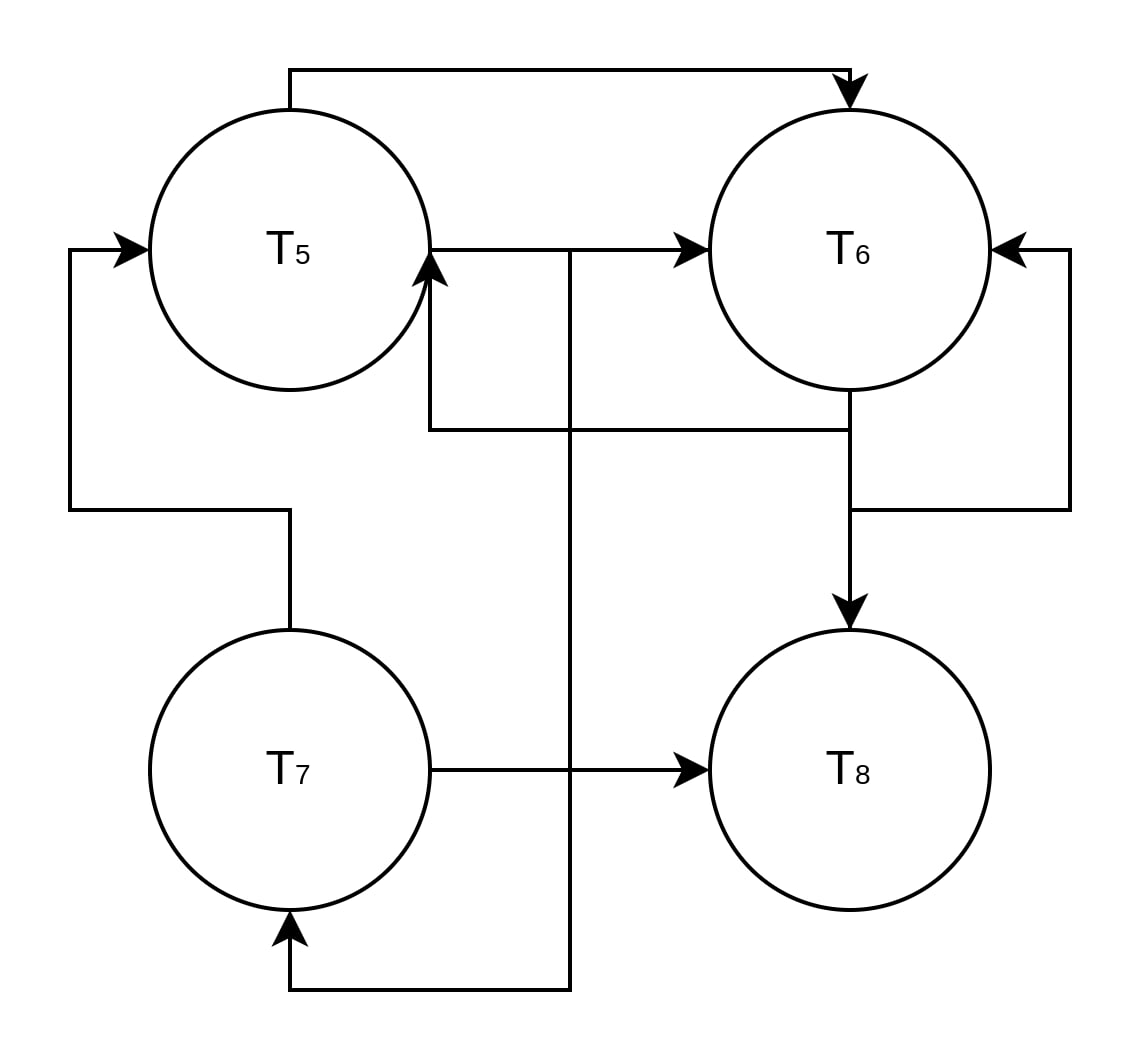
\includegraphics[width=0.3\textwidth]{umls/exp1_serializable_graph.jpg}
    \caption{گراف تراکنش‌ها و ایجاد ارتباطات حلقه دار}
    \label{fig: diagram}
\end{figure}

در این مثال برای حذف حلقه می‌تواند یکی یکی تراکنش‌های مورد نظر را بررسی کرد و در
صورت حذف یکی از تراکنش‌ها حلقه حذف شد می‌توان آن را نتیجه گرفت و اعلام کرد این
تراکنش‌ها باهم سازگارند و برخورد ایجاد نمی‌کنند. در نهایت سیستم DBM تصمیم به
اجرای تراکنش‌ها خواهد کرد.

\begin{figure}[H]
    \centering
    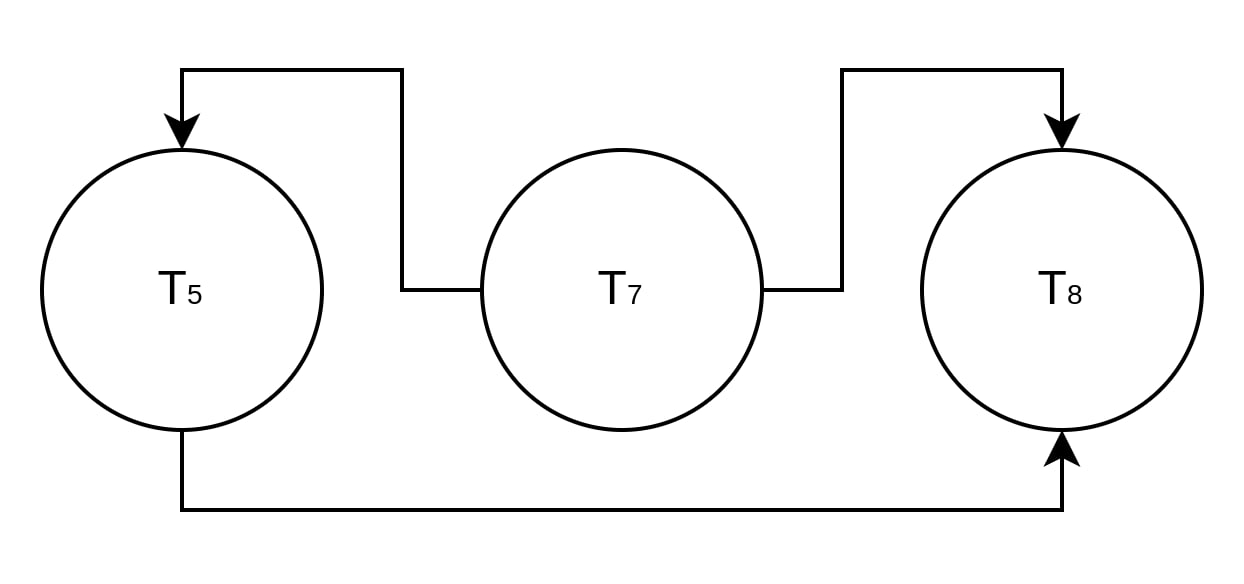
\includegraphics[width=0.3\textwidth]{umls/exp1_solved.jpg}
    \caption{تراکنش حذف شده و ایجاد گرافی بدون حلقه}
    \label{fig: diagram}
\end{figure}

\subsubsection{پی در پی پذیری در دید یا \lr{View equivalent}}

زمانی می‌گوییم پی در پی پذیری در دید برقرار است که نتایج \underline{یکسانی} در
سیستم DBM با یک زمان‌بندی پی در پی داشته باشیم.

\subsubsection*{بررسی پی در پی پذیری در دید به ۲ روش می‌تواند انجام شود}

\begin{enumerate}
    \item بررسی $R_{initial}<...<R_{middle}<...<W_{final}$
    \item استفاده از روش \lr{Read from}
\end{enumerate}

سه قاعده اصلی پی در پی پذیری در دید:

\begin{enumerate}
    \item برای هر داده Q تراکنشی که در S مقدار اولیه داده‌ای Q  را می‌خواند در
    S' هم همان تراکنش اولیه مقدار Q را بخواند (خواندن‌های اولیه)
    \item برای هر داده‌ Q اگر $t_{i}$ در S داده‌ Q را از $t_{j}$ می‌خواند، در S'
    هم $t_{i}$ همان داده‌ را از $t_{j}$ بخواند. (خواندن‌های میانی)
    \item برای هر داده Q آخرین تراکنشی از S که روی Q می‌نویسد در S' هم همان
    تراکنش نوشتن پایانی را روی Q انجام دهد. (نوشتن‌های پایانی)
\end{enumerate}

نکته: یک زمانبندی پی در پی پذیر در دید است، هنگامی که معادل در دید با یک
زمانبندی پی در پی پذیر باشد که نتایج درستی را منعکس کند.

\subsubsection{مثال اول پی در پی پذیری در دید}

\begin{LTR}
    \begin{table}[h]
        \centering
        \begin{RTL}
            \caption{پی در پی پذیری در دید}
        \end{RTL}
        \begin{tabular}{c|c|c|c|c|c}
            $T_{5}$ & & & W(Q) & & \\ \hline
            $T_{6}$ & R(Q) & & & &  \\ \hline
            $T_{7}$ & & W(Q) & & & W(Q) \\ \hline
            $T_{8}$ & & & & R(Q) & \\
        \end{tabular}
    \end{table}
\end{LTR}

پی در پی پذیر در دید است چرا که فرایند خواندن اولیه و عملیات میانی و در نهایت
نوشتن پایانی را دارا می‌باشد.

\begin{LTR}
    $T_{6}$ > ....... > $T_{7}$

    $T_{6}$ > $T_{5}$ > $T_{8}$ > $T_{7}$
\end{LTR}

اما پی در پی پذیر در برخورد نیست چرا که بین تراکنش $T_{7}$ و $T_{8}$ یک حلقه
ایجاد می‌شود و می‌تواند عاملی در برخورد باشد.

\subsubsection{مثال دوم پی در پی پذیری در دید}

\begin{LTR}
    \begin{table}[h]
        \centering
        \begin{RTL}
            \caption{پی در پی پذیری در دید}
        \end{RTL}
        \begin{tabular}{c|c|c|c}
            $T_{3}$ & R(Q) & & W(Q) C \\ \hline
            $T_{4}$ & & W(Q) C &  \\ \hline
            $T_{5}$ & & & W(Q) C \\
        \end{tabular}
    \end{table}
\end{LTR}

جواب: این مثال پی در پی پذیر در دید است:

\begin{LTR}
    $T_{3}$ > ....... > $T_{5}$
\end{LTR}

چرا که در $T_{3}$ خواندن‌های اولیه صورت گرفته، در $T_{4}$ و زمان میانی $T_{3}$
عملیات میانی نوشتن رخ داده است. در انتها در تراکنش $T_{5}$ مطابق با قانون پی در
پی پذیری در دید نوشتن پایانی انجام شده است.

اما پی در پی پذیر در برخورد نیست چرا که در میان تراکنش‌ها حلقه رخ داده است.

\begin{figure}[H]
    \centering
    \caption{فاقد پی در پی پذیری تراکنش‌ها در برخورد}
    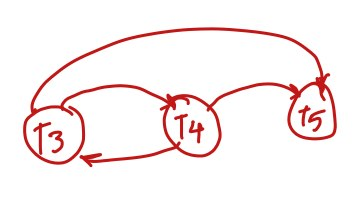
\includegraphics[width=0.4\textwidth]{umls/vsr_exp_2.jpg}
\end{figure}

\subsubsection*{نکته}

اگر یک زمانبندی در برخورد پی در پی پذیر بود می‌تواند در دید هم پی در پی پذیر
باشد. اما می‌تواند سناریویی مطرح شود که در آن تنها پی در پی پذیر در دید باشد ولی
در برخورد نباشد.

\subsubsection{نمادگزاری}

کامپیوتر چگونه پی در پی پذیری در دید را متوجه می‌شود؟ با استفاده از نمادگزاری
(خواندن از). برای یک زمانبندی، مجموعه‌ای از (خواندن از‌)ها را تشکیل می‌دهیم. این
مجموعه باید با مجموعه خواندن از‌ها در یک زمانبندی پی در پی دیگر یکسان باشد تا در
دید هم پی در پی پذیر باشد. در این روش مدت زمان اجرا \footnote{Runtime} برای
کامپیوتر طولانی است و اجرای آن برای کامپیوتر بهینه نیست.

مثال:

\begin{LTR}
$S = r_{2}(x), w_{2}(x), r_{1}(x), r_{1}(y), r_{2}(y), w_{2}(y), c_{1}, c_{2} $
\end{LTR}

\subsubsection*{بدست آوردن مرجع اصلی}

\begin{LTR}
$RF(S) = (T_{0}, x, T_{2}), (T_{2}, x, T_{1}), (T_{0}, y, T_{1}), (T_{0}, y, T_{2})$
\end{LTR}

\subsubsection*{بدست آوردن $T_{1} < T_{2}$}

در این مرحله ابتدا تراکنش‌های زمانبندی اول انجام می‌شود و سپس تراکنش‌های زمانبندی دوم:

\begin{LTR}
$T_{1} < T_{2}$ = $r_{1}(x), r_{1}(y), c_{1}, r_{2}(x), w_{2}(x), r_{2}(y), w_{2}(y), c_{2}$
\end{LTR}

بدست آوردن RF به وسیله ترتیب زمانبندی بالا:

\begin{LTR}
$RF(T_{1} < T_{2}) = (T_{0}, x, T_{1}), (T_{0}, y, T_{1}), (T_{0}, x, T_{2}), (T_{0}, y, T_{2})$
\end{LTR}

\subsubsection*{بدست آوردن $T_{2} < T_{1}$}

در این مرحله زمانبندی دوم در ابتدا و سپس زمانبندی اول بعد از آن اجرا می‌شود:

\begin{LTR}
$T_{2} < T_{1}$ = $r_{2}(x), w_{2}(x), r_{2}(y), w_{2}(y), c_{2}, r_{1}(x), r_{1}(y), c_{1}$
\end{LTR}

بدست آوردن RF به وسیله ترتیب زمانبندی جدید بالا:

\begin{LTR}
$RF(T_{2} < T_{1}) = (T_{0}, x, T_{2}), (T_{0}, y, T_{2}), (T_{2}, x, T_{1}), (T_{2}, y, T_{1})$
\end{LTR}

بعد از نوشتن عملیات بالا متوجه خواهید شد که هیچ کدام از $RF(T_{1} < T_{2})$ و
$RF(T_{2} < T_{1})$ با مرجع اصلی $RF(S)$ که در ابتدا نوشتیم برابر نیست.

\newpage